\documentclass[border=10pt]{standalone}
\usepackage{tikz}\usepackage{amsmath}\usetikzlibrary{arrows.meta}
\begin{document}
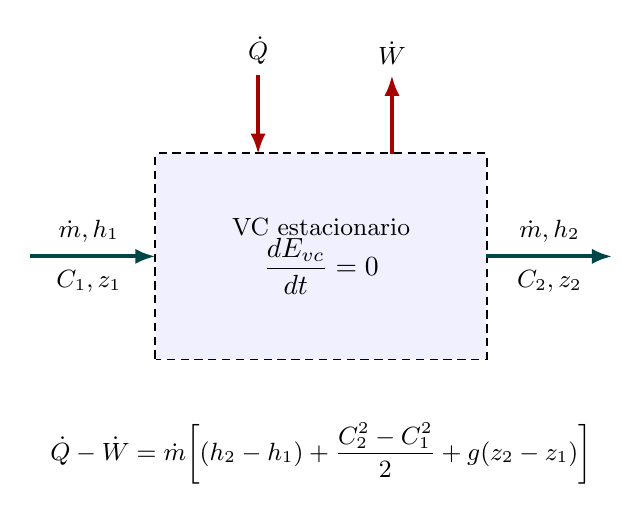
\begin{tikzpicture}[line width=1pt,>={Latex[length=2.6mm]}]
  \draw[densely dashed,line width=1.2pt] (0,0) rectangle (4.2,2.6);
  \fill[blue!6] (0,0) rectangle (4.2,2.6);
  \node[align=center] at (2.1,1.3){\small VC estacionario\\$\dfrac{dE_{vc}}{dt}=0$};
  % una entrada, una salida
  \draw[->,teal!55!black,line width=1.5pt] (-1.6,1.3)--(0,1.3);
  \node[above] at (-0.85,1.35){\small $\dot m,h_1$}; \node[below] at (-0.85,1.25){\small $C_1,z_1$};
  \draw[->,teal!55!black,line width=1.5pt] (4.2,1.3)--(5.8,1.3);
  \node[above] at (5.0,1.35){\small $\dot m,h_2$}; \node[below] at (5.0,1.25){\small $C_2,z_2$};
  % Q y W
  \draw[->,red!65!black,line width=1.3pt] (1.3,3.6)--(1.3,2.6); \node[above] at (1.3,3.6){\small $\dot Q$};
  \draw[->,red!65!black,line width=1.3pt] (3.0,2.6)--(3.0,3.6); \node[above] at (3.0,3.6){\small $\dot W$};
  \node[align=center] at (2.1,-1.2){\small $\dot Q-\dot W=\dot m\!\left[(h_2-h_1)+\dfrac{C_2^2-C_1^2}{2}+g(z_2-z_1)\right]$};
\end{tikzpicture}
\end{document}
